\documentclass[bachelorscriptie]{uvamath}%use option "english" for an English thesis
%Alle mogelijke opties zijn: complatex, tweedejaarsproject, bachelorscriptie, dubaWI, dubaWN

\usepackage[dutch]{babel} %Remark: use the same language for uvamath and babel
\usepackage{graphicx}
\usepackage[pdfborder={0 0 0}]{hyperref}
\usepackage{lipsum}

\title{Lossless Image Coding}
\author[henk@science.uva.nl, 6127901]{Henk de Vries}
%\author[ingrid@science.uva.nl, 6123102]{Ingrid de Vries}

\supervisors{prof.\ dr.\ Carl Friedrich Gauss}
%\supervisors{prof.\ dr.\ Emmy Noether}
\secondgrader{dr.\ Karl Weierstrass}
%\secondgrader{prof. dr.\ Leonhard Euler}
\coverimage{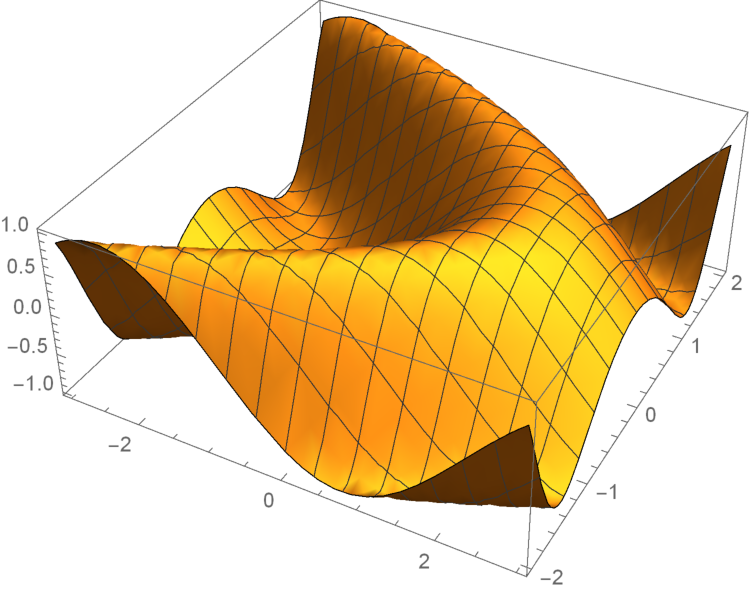
\includegraphics[scale=0.8]{figuur.pdf}}

\begin{document}
\maketitle

\begin{abstract}
Schrijf een samenvatting van hoogstens een halve bladzijde waarin je kort uitlegt wat je hebt gedaan. De samenvatting schrijf je als laatste. Je mag er vanuit gaan dat je docent de lezer is.
\end{abstract}

\tableofcontents

\chapter{Inleiding}
Vertel iets over je artikel, noem je vraagstelling. Richt je tekst op medestudenten. (Richtlijn 2 bladzijden).

\chapter{Eliminatie}
\lipsum[1-3]

\chapter{Differenti\"eren en integreren}
\lipsum[1-3]

\chapter{Conclusie}
\lipsum[1-3]


\clearpage%to fix page numbering in ToC
\addcontentsline{toc}{chapter}{Bibliografie}
\begin{thebibliography}{}
\bibitem{Zaal95}
Zaal, Chris. ``Explicit complete curves in the moduli space of curves of genus three." Geometriae dedicata 56.2 (1995): 185-196.
\end{thebibliography}

\clearpage%to fix page numbering in ToC
\chapter*{Populaire samenvatting}
\addcontentsline{toc}{chapter}{Populaire samenvatting}
\lipsum[1-2]

\appendix

\chapter{Lineaire Algebra}
\lipsum[1-3]

\end{document}